\chapter{Statistické okénko}
\label{statistika}

\begin{center}

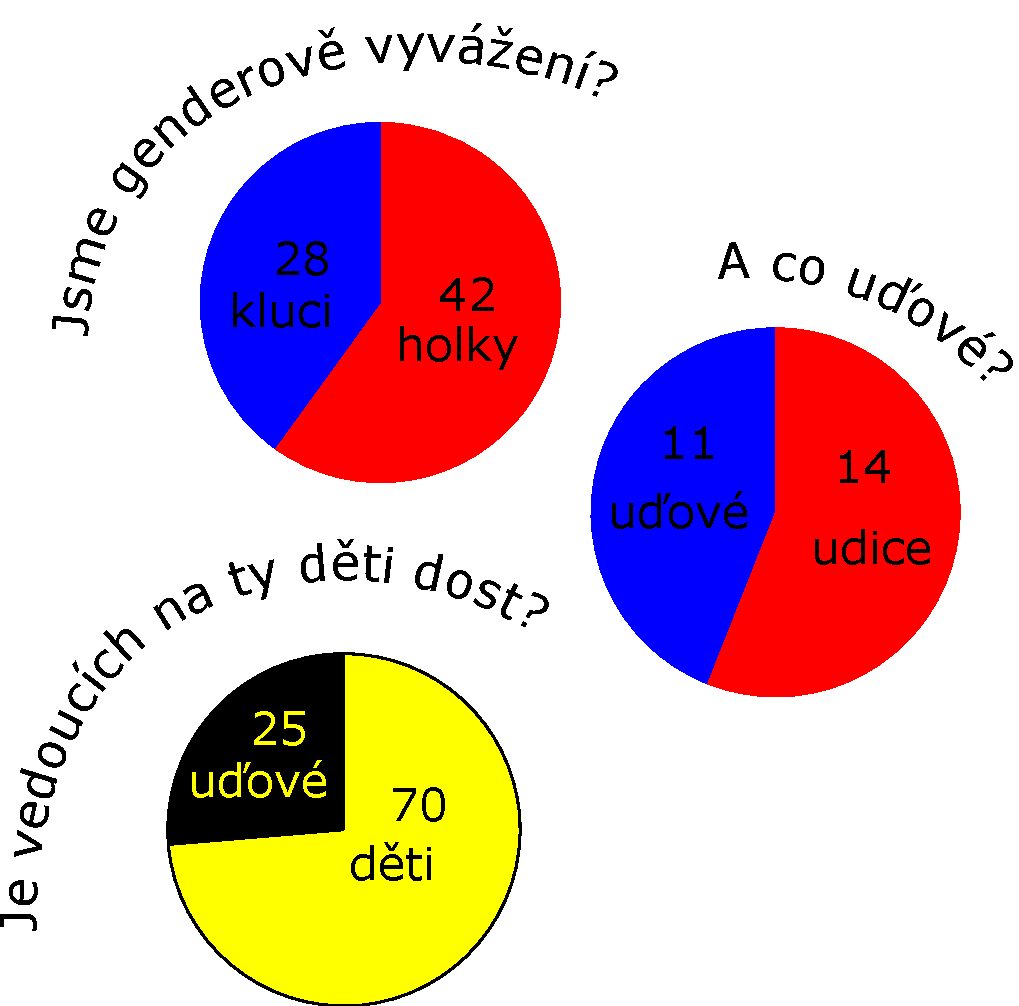
\includegraphics[width=12cm]{img/statistika/grafy-kolacove.pdf}

\end{center}


\clearpage

Pro ještě větší milovníky statistiky přikládáme analýzu věku a doby členství v oddíle zpracované jako histogramy. Na Obr. \ref{fig:vek} je rozdělení věku (platné jeden týden před vánočním večírkem). Na Obr. \ref{fig:clen} je rozdělení počtu let v oddíle.

Pro upřesnění: roky počítáme od nuly. Data pochází ze skautisu, nepřesnosti jsou (obvláště u nových členů) možné. Grafy jsou na ose x zaříznuté a neobsahují tedy všechny hodnoty (někteří exuďové 24 let v oddíle). V těchto histogramech nebyli rozlišeni uďové od dětí.

\begin{figure}[!ht]
  \begin{center}
    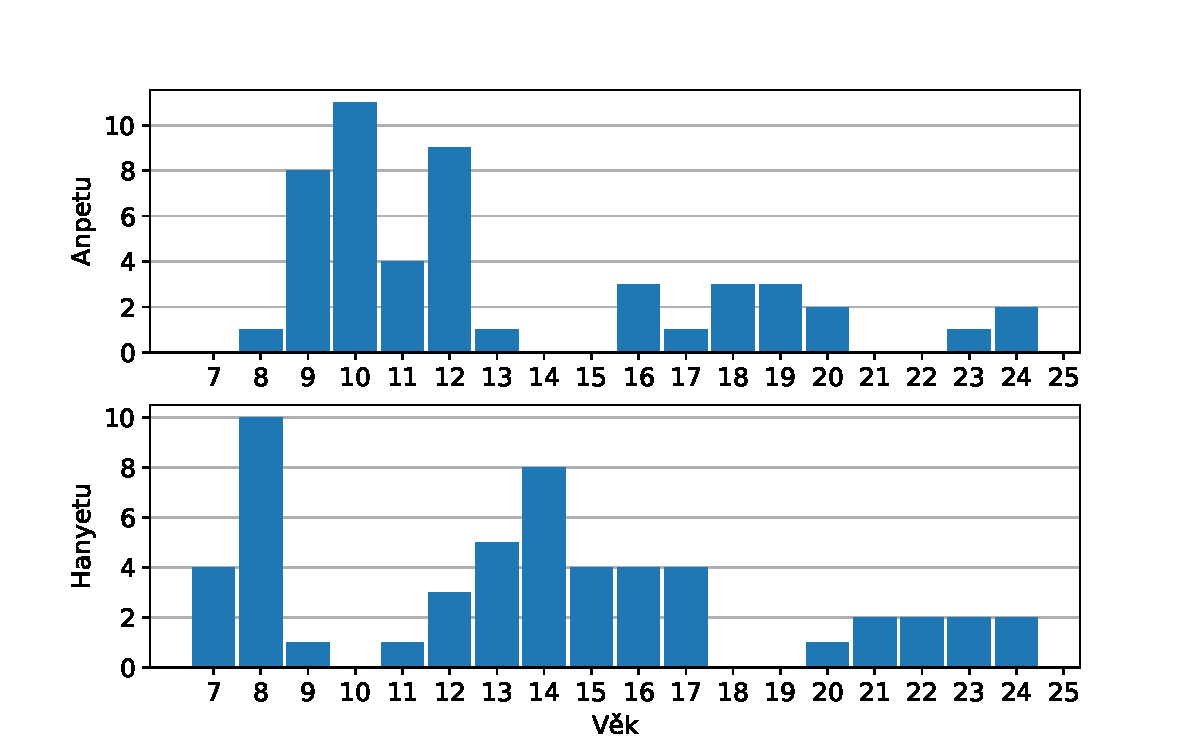
\includegraphics[width=0.75\textwidth]{statistika/hist_vek.pdf}
  \end{center}
  \caption{Histogram věku účastníků}
  \label{fig:vek}
\end{figure}


\begin{figure}[!ht]
  \begin{center}
    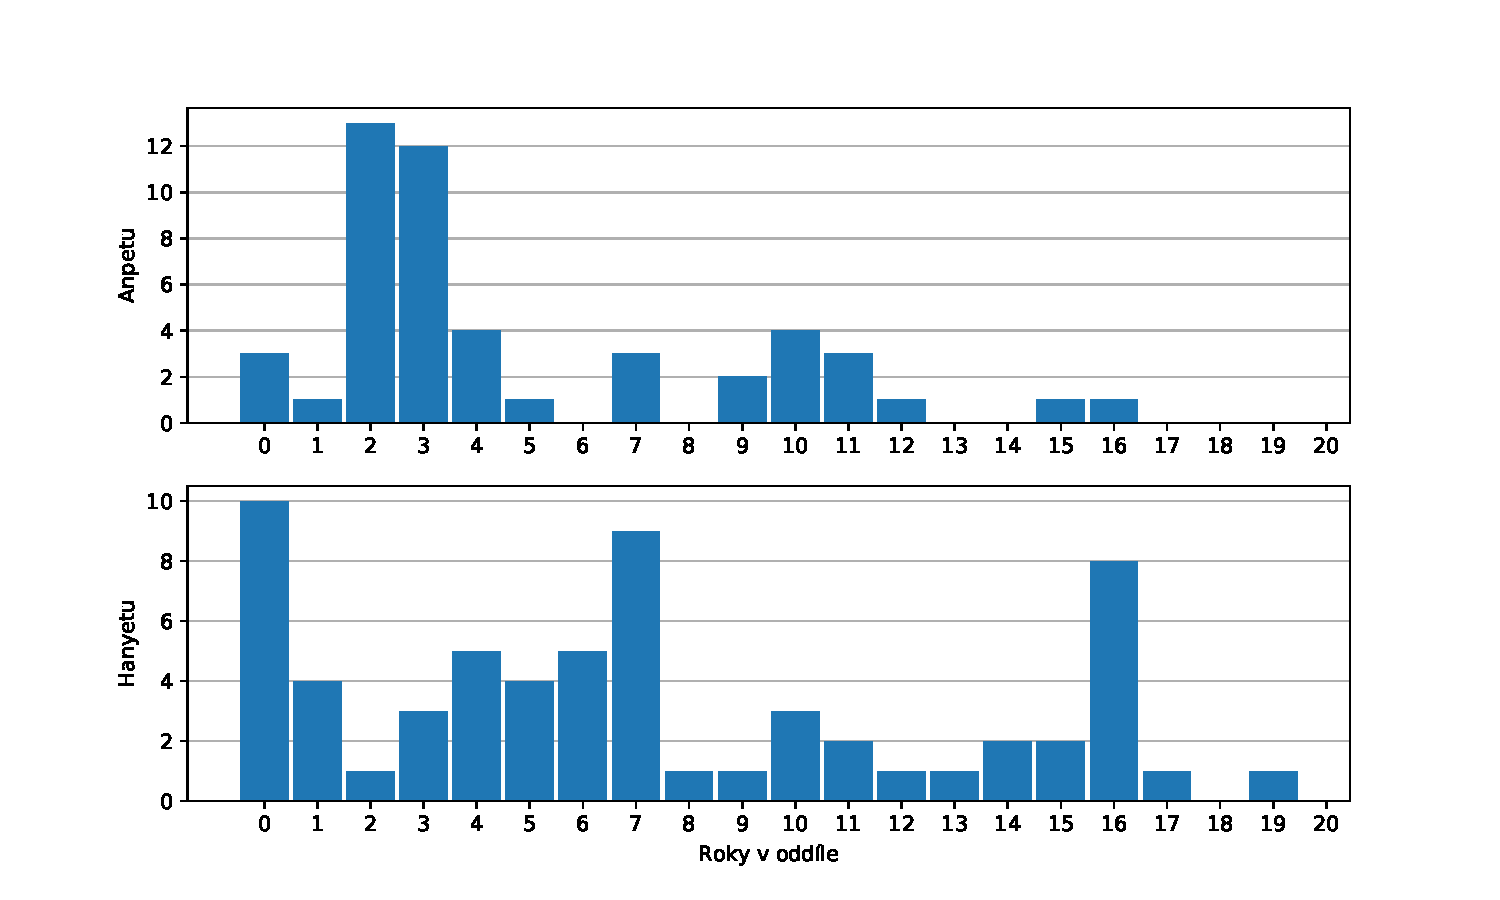
\includegraphics[width=0.75\textwidth]{statistika/hist_clen.pdf}
  \end{center}
  \caption{Histogram doby člesntví v oddíle}
  \label{fig:clen}
\end{figure}

\clearpage
